\PassOptionsToPackage{unicode=true}{hyperref} % options for packages loaded elsewhere
\PassOptionsToPackage{hyphens}{url}
%
\documentclass[]{article}
\usepackage{lmodern}
\usepackage{amssymb,amsmath}
\usepackage{ifxetex,ifluatex}
\usepackage{fixltx2e} % provides \textsubscript
\ifnum 0\ifxetex 1\fi\ifluatex 1\fi=0 % if pdftex
  \usepackage[T1]{fontenc}
  \usepackage[utf8]{inputenc}
  \usepackage{textcomp} % provides euro and other symbols
\else % if luatex or xelatex
  \usepackage{unicode-math}
  \defaultfontfeatures{Ligatures=TeX,Scale=MatchLowercase}
\fi
% use upquote if available, for straight quotes in verbatim environments
\IfFileExists{upquote.sty}{\usepackage{upquote}}{}
% use microtype if available
\IfFileExists{microtype.sty}{%
\usepackage[]{microtype}
\UseMicrotypeSet[protrusion]{basicmath} % disable protrusion for tt fonts
}{}
\IfFileExists{parskip.sty}{%
\usepackage{parskip}
}{% else
\setlength{\parindent}{0pt}
\setlength{\parskip}{6pt plus 2pt minus 1pt}
}
\usepackage{hyperref}
\hypersetup{
            pdftitle={Assignment 7: GLMs week 2 (Linear Regression and beyond)},
            pdfauthor={Cristiana Falvo},
            pdfborder={0 0 0},
            breaklinks=true}
\urlstyle{same}  % don't use monospace font for urls
\usepackage[margin=2.54cm]{geometry}
\usepackage{color}
\usepackage{fancyvrb}
\newcommand{\VerbBar}{|}
\newcommand{\VERB}{\Verb[commandchars=\\\{\}]}
\DefineVerbatimEnvironment{Highlighting}{Verbatim}{commandchars=\\\{\}}
% Add ',fontsize=\small' for more characters per line
\usepackage{framed}
\definecolor{shadecolor}{RGB}{248,248,248}
\newenvironment{Shaded}{\begin{snugshade}}{\end{snugshade}}
\newcommand{\AlertTok}[1]{\textcolor[rgb]{0.94,0.16,0.16}{#1}}
\newcommand{\AnnotationTok}[1]{\textcolor[rgb]{0.56,0.35,0.01}{\textbf{\textit{#1}}}}
\newcommand{\AttributeTok}[1]{\textcolor[rgb]{0.77,0.63,0.00}{#1}}
\newcommand{\BaseNTok}[1]{\textcolor[rgb]{0.00,0.00,0.81}{#1}}
\newcommand{\BuiltInTok}[1]{#1}
\newcommand{\CharTok}[1]{\textcolor[rgb]{0.31,0.60,0.02}{#1}}
\newcommand{\CommentTok}[1]{\textcolor[rgb]{0.56,0.35,0.01}{\textit{#1}}}
\newcommand{\CommentVarTok}[1]{\textcolor[rgb]{0.56,0.35,0.01}{\textbf{\textit{#1}}}}
\newcommand{\ConstantTok}[1]{\textcolor[rgb]{0.00,0.00,0.00}{#1}}
\newcommand{\ControlFlowTok}[1]{\textcolor[rgb]{0.13,0.29,0.53}{\textbf{#1}}}
\newcommand{\DataTypeTok}[1]{\textcolor[rgb]{0.13,0.29,0.53}{#1}}
\newcommand{\DecValTok}[1]{\textcolor[rgb]{0.00,0.00,0.81}{#1}}
\newcommand{\DocumentationTok}[1]{\textcolor[rgb]{0.56,0.35,0.01}{\textbf{\textit{#1}}}}
\newcommand{\ErrorTok}[1]{\textcolor[rgb]{0.64,0.00,0.00}{\textbf{#1}}}
\newcommand{\ExtensionTok}[1]{#1}
\newcommand{\FloatTok}[1]{\textcolor[rgb]{0.00,0.00,0.81}{#1}}
\newcommand{\FunctionTok}[1]{\textcolor[rgb]{0.00,0.00,0.00}{#1}}
\newcommand{\ImportTok}[1]{#1}
\newcommand{\InformationTok}[1]{\textcolor[rgb]{0.56,0.35,0.01}{\textbf{\textit{#1}}}}
\newcommand{\KeywordTok}[1]{\textcolor[rgb]{0.13,0.29,0.53}{\textbf{#1}}}
\newcommand{\NormalTok}[1]{#1}
\newcommand{\OperatorTok}[1]{\textcolor[rgb]{0.81,0.36,0.00}{\textbf{#1}}}
\newcommand{\OtherTok}[1]{\textcolor[rgb]{0.56,0.35,0.01}{#1}}
\newcommand{\PreprocessorTok}[1]{\textcolor[rgb]{0.56,0.35,0.01}{\textit{#1}}}
\newcommand{\RegionMarkerTok}[1]{#1}
\newcommand{\SpecialCharTok}[1]{\textcolor[rgb]{0.00,0.00,0.00}{#1}}
\newcommand{\SpecialStringTok}[1]{\textcolor[rgb]{0.31,0.60,0.02}{#1}}
\newcommand{\StringTok}[1]{\textcolor[rgb]{0.31,0.60,0.02}{#1}}
\newcommand{\VariableTok}[1]{\textcolor[rgb]{0.00,0.00,0.00}{#1}}
\newcommand{\VerbatimStringTok}[1]{\textcolor[rgb]{0.31,0.60,0.02}{#1}}
\newcommand{\WarningTok}[1]{\textcolor[rgb]{0.56,0.35,0.01}{\textbf{\textit{#1}}}}
\usepackage{graphicx,grffile}
\makeatletter
\def\maxwidth{\ifdim\Gin@nat@width>\linewidth\linewidth\else\Gin@nat@width\fi}
\def\maxheight{\ifdim\Gin@nat@height>\textheight\textheight\else\Gin@nat@height\fi}
\makeatother
% Scale images if necessary, so that they will not overflow the page
% margins by default, and it is still possible to overwrite the defaults
% using explicit options in \includegraphics[width, height, ...]{}
\setkeys{Gin}{width=\maxwidth,height=\maxheight,keepaspectratio}
\setlength{\emergencystretch}{3em}  % prevent overfull lines
\providecommand{\tightlist}{%
  \setlength{\itemsep}{0pt}\setlength{\parskip}{0pt}}
\setcounter{secnumdepth}{0}
% Redefines (sub)paragraphs to behave more like sections
\ifx\paragraph\undefined\else
\let\oldparagraph\paragraph
\renewcommand{\paragraph}[1]{\oldparagraph{#1}\mbox{}}
\fi
\ifx\subparagraph\undefined\else
\let\oldsubparagraph\subparagraph
\renewcommand{\subparagraph}[1]{\oldsubparagraph{#1}\mbox{}}
\fi

% set default figure placement to htbp
\makeatletter
\def\fps@figure{htbp}
\makeatother


\title{Assignment 7: GLMs week 2 (Linear Regression and beyond)}
\author{Cristiana Falvo}
\date{}

\begin{document}
\maketitle

\hypertarget{overview}{%
\subsection{OVERVIEW}\label{overview}}

This exercise accompanies the lessons in Environmental Data Analytics on
generalized linear models.

\hypertarget{directions}{%
\subsection{Directions}\label{directions}}

\begin{enumerate}
\def\labelenumi{\arabic{enumi}.}
\tightlist
\item
  Change ``Student Name'' on line 3 (above) with your name.
\item
  Work through the steps, \textbf{creating code and output} that fulfill
  each instruction.
\item
  Be sure to \textbf{answer the questions} in this assignment document.
\item
  When you have completed the assignment, \textbf{Knit} the text and
  code into a single PDF file.
\item
  After Knitting, submit the completed exercise (PDF file) to the
  dropbox in Sakai. Add your last name into the file name (e.g.,
  ``Salk\_A06\_GLMs\_Week1.Rmd'') prior to submission.
\end{enumerate}

The completed exercise is due on Tuesday, February 25 at 1:00 pm.

\hypertarget{set-up-your-session}{%
\subsection{Set up your session}\label{set-up-your-session}}

\begin{enumerate}
\def\labelenumi{\arabic{enumi}.}
\item
  Set up your session. Check your working directory, load the tidyverse,
  nlme, and piecewiseSEM packages, import the \emph{raw} NTL-LTER raw
  data file for chemistry/physics, and import the processed litter
  dataset. You will not work with dates, so no need to format your date
  columns this time.
\item
  Build a ggplot theme and set it as your default theme.
\end{enumerate}

\begin{Shaded}
\begin{Highlighting}[]
\CommentTok{#1}
\KeywordTok{getwd}\NormalTok{()}
\end{Highlighting}
\end{Shaded}

\begin{verbatim}
## [1] "/Users/cristiana/Documents/Duke/DataAnalytics/Environmental_Data_Analytics_2020"
\end{verbatim}

\begin{Shaded}
\begin{Highlighting}[]
\KeywordTok{library}\NormalTok{(tidyverse)}
\end{Highlighting}
\end{Shaded}

\begin{verbatim}
## -- Attaching packages ---------------------------------------------------------------- tidyverse 1.3.0 --
\end{verbatim}

\begin{verbatim}
## v ggplot2 3.2.1     v purrr   0.3.3
## v tibble  2.1.3     v dplyr   0.8.3
## v tidyr   1.0.0     v stringr 1.4.0
## v readr   1.3.1     v forcats 0.4.0
\end{verbatim}

\begin{verbatim}
## -- Conflicts ------------------------------------------------------------------- tidyverse_conflicts() --
## x dplyr::filter() masks stats::filter()
## x dplyr::lag()    masks stats::lag()
\end{verbatim}

\begin{Shaded}
\begin{Highlighting}[]
\KeywordTok{library}\NormalTok{(nlme)}
\end{Highlighting}
\end{Shaded}

\begin{verbatim}
## 
## Attaching package: 'nlme'
\end{verbatim}

\begin{verbatim}
## The following object is masked from 'package:dplyr':
## 
##     collapse
\end{verbatim}

\begin{Shaded}
\begin{Highlighting}[]
\KeywordTok{library}\NormalTok{(piecewiseSEM)}
\end{Highlighting}
\end{Shaded}

\begin{verbatim}
## Registered S3 methods overwritten by 'lme4':
##   method                          from
##   cooks.distance.influence.merMod car 
##   influence.merMod                car 
##   dfbeta.influence.merMod         car 
##   dfbetas.influence.merMod        car
\end{verbatim}

\begin{verbatim}
## 
##   This is piecewiseSEM version 2.1.0.
## 
## 
##   Questions or bugs can be addressed to <LefcheckJ@si.edu>.
\end{verbatim}

\begin{Shaded}
\begin{Highlighting}[]
\CommentTok{# to visualize linear reg}
\KeywordTok{require}\NormalTok{(ggiraph)}
\end{Highlighting}
\end{Shaded}

\begin{verbatim}
## Loading required package: ggiraph
\end{verbatim}

\begin{Shaded}
\begin{Highlighting}[]
\KeywordTok{require}\NormalTok{(ggiraphExtra)}
\end{Highlighting}
\end{Shaded}

\begin{verbatim}
## Loading required package: ggiraphExtra
\end{verbatim}

\begin{Shaded}
\begin{Highlighting}[]
\KeywordTok{require}\NormalTok{(plyr)}
\end{Highlighting}
\end{Shaded}

\begin{verbatim}
## Loading required package: plyr
\end{verbatim}

\begin{verbatim}
## ------------------------------------------------------------------------------
\end{verbatim}

\begin{verbatim}
## You have loaded plyr after dplyr - this is likely to cause problems.
## If you need functions from both plyr and dplyr, please load plyr first, then dplyr:
## library(plyr); library(dplyr)
\end{verbatim}

\begin{verbatim}
## ------------------------------------------------------------------------------
\end{verbatim}

\begin{verbatim}
## 
## Attaching package: 'plyr'
\end{verbatim}

\begin{verbatim}
## The following objects are masked from 'package:dplyr':
## 
##     arrange, count, desc, failwith, id, mutate, rename, summarise,
##     summarize
\end{verbatim}

\begin{verbatim}
## The following object is masked from 'package:purrr':
## 
##     compact
\end{verbatim}

\begin{Shaded}
\begin{Highlighting}[]
\CommentTok{# data}
\NormalTok{chem_phys <-}\StringTok{ }\KeywordTok{read.csv}\NormalTok{(}\StringTok{"/Users/cristiana/Documents/Duke/DataAnalytics/Environmental_Data_Analytics_2020/Data/Raw/NTL-LTER_Lake_ChemistryPhysics_Raw.csv"}\NormalTok{)}
\NormalTok{litter <-}\StringTok{ }\KeywordTok{read.csv}\NormalTok{(}\StringTok{"/Users/cristiana/Documents/Duke/DataAnalytics/Environmental_Data_Analytics_2020/Data/Processed/NEON_NIWO_Litter_mass_trap_Processed.csv"}\NormalTok{)}

\CommentTok{#2}
\NormalTok{mytheme <-}\StringTok{ }\KeywordTok{theme_classic}\NormalTok{(}\DataTypeTok{base_size =} \DecValTok{14}\NormalTok{) }\OperatorTok{+}
\StringTok{  }\KeywordTok{theme}\NormalTok{(}\DataTypeTok{axis.text =} \KeywordTok{element_text}\NormalTok{(}\DataTypeTok{color =} \StringTok{"black"}\NormalTok{), }
        \DataTypeTok{legend.position =} \StringTok{"top"}\NormalTok{)}
\KeywordTok{theme_set}\NormalTok{(mytheme)}
\end{Highlighting}
\end{Shaded}

\hypertarget{ntl-lter-test}{%
\subsection{NTL-LTER test}\label{ntl-lter-test}}

Research question: What is the best set of predictors for lake
temperatures in July across the monitoring period at the North Temperate
Lakes LTER?

\# is this asking, what's the optimal combination of variables (aic..)
to predict lake temps in july?

\begin{enumerate}
\def\labelenumi{\arabic{enumi}.}
\setcounter{enumi}{2}
\tightlist
\item
  Wrangle your NTL-LTER dataset with a pipe function so that it contains
  only the following criteria:
\end{enumerate}

\begin{itemize}
\tightlist
\item
  Only dates in July (hint: use the daynum column). No need to consider
  leap years. (182-212)
\item
  Only the columns: lakename, year4, daynum, depth, temperature\_C
  (select())
\item
  Only complete cases (i.e., remove NAs) (na.omit(data))
\end{itemize}

\begin{enumerate}
\def\labelenumi{\arabic{enumi}.}
\setcounter{enumi}{3}
\tightlist
\item
  Run an AIC to determine what set of explanatory variables (year4,
  daynum, depth) is best suited to predict temperature. Run a multiple
  regression on the recommended set of variables. \# run aic, this will
  give optimal combo of variables \# with this optimal set of vars, run
  a `multiple regression'
\end{enumerate}

\begin{Shaded}
\begin{Highlighting}[]
\CommentTok{#3 get subset of data}
\NormalTok{chem_phys_subset <-}\StringTok{ }
\StringTok{  }\NormalTok{chem_phys }\OperatorTok
\StringTok{  }\KeywordTok{filter}\NormalTok{(daynum }\OperatorTok{>=}\StringTok{ }\DecValTok{182} \OperatorTok{&}\StringTok{ }\NormalTok{daynum }\OperatorTok{<=}\StringTok{ }\DecValTok{212}\NormalTok{) }\OperatorTok
\StringTok{  }\KeywordTok{select}\NormalTok{(lakename, year4, daynum, depth, temperature_C) }\OperatorTok\StringTok{ }\CommentTok{# 10,836}
\StringTok{  }\KeywordTok{na.omit}\NormalTok{()}

\CommentTok{#4 run AIC to determine best combination of predictor variables}
\NormalTok{temp_AIC <-}\StringTok{ }\KeywordTok{lm}\NormalTok{(}\DataTypeTok{data =}\NormalTok{ chem_phys_subset, temperature_C }\OperatorTok{~}\StringTok{ }\NormalTok{year4 }\OperatorTok{+}\StringTok{ }\NormalTok{daynum }\OperatorTok{+}\StringTok{ }\NormalTok{depth) }
\KeywordTok{step}\NormalTok{(temp_AIC) }
\end{Highlighting}
\end{Shaded}

\begin{verbatim}
## Start:  AIC=26016.31
## temperature_C ~ year4 + daynum + depth
## 
##          Df Sum of Sq    RSS   AIC
## <none>                141118 26016
## - year4   1        80 141198 26020
## - daynum  1      1333 142450 26106
## - depth   1    403925 545042 39151
\end{verbatim}

\begin{verbatim}
## 
## Call:
## lm(formula = temperature_C ~ year4 + daynum + depth, data = chem_phys_subset)
## 
## Coefficients:
## (Intercept)        year4       daynum        depth  
##    -6.45556      0.01013      0.04134     -1.94726
\end{verbatim}

\begin{Shaded}
\begin{Highlighting}[]
\NormalTok{temp_model <-}\StringTok{ }\KeywordTok{lm}\NormalTok{(}\DataTypeTok{data =}\NormalTok{ chem_phys_subset, temperature_C }\OperatorTok{~}\StringTok{ }\NormalTok{year4 }\OperatorTok{+}\StringTok{ }\NormalTok{daynum }\OperatorTok{+}\StringTok{ }\NormalTok{depth)}
\KeywordTok{summary}\NormalTok{(temp_model) }
\end{Highlighting}
\end{Shaded}

\begin{verbatim}
## 
## Call:
## lm(formula = temperature_C ~ year4 + daynum + depth, data = chem_phys_subset)
## 
## Residuals:
##     Min      1Q  Median      3Q     Max 
## -9.6517 -2.9937  0.0855  2.9692 13.6171 
## 
## Coefficients:
##              Estimate Std. Error  t value Pr(>|t|)    
## (Intercept) -6.455560   8.638808   -0.747   0.4549    
## year4        0.010131   0.004303    2.354   0.0186 *  
## daynum       0.041336   0.004315    9.580   <2e-16 ***
## depth       -1.947264   0.011676 -166.782   <2e-16 ***
## ---
## Signif. codes:  0 '***' 0.001 '**' 0.01 '*' 0.05 '.' 0.1 ' ' 1
## 
## Residual standard error: 3.811 on 9718 degrees of freedom
## Multiple R-squared:  0.7417, Adjusted R-squared:  0.7417 
## F-statistic:  9303 on 3 and 9718 DF,  p-value: < 2.2e-16
\end{verbatim}

\begin{Shaded}
\begin{Highlighting}[]
\CommentTok{# is this model the multiple regression?}
\CommentTok{# is there a way to visualize it?}
  \CommentTok{# can visualize individual relatinships (switch between year, daynum, depth - depth is only one with noteable correlation)}
\NormalTok{linear_reg_rel <-}\StringTok{ }
\StringTok{  }\KeywordTok{ggplot}\NormalTok{(chem_phys_subset, }\KeywordTok{aes}\NormalTok{(}\DataTypeTok{x =}\NormalTok{ depth, }\DataTypeTok{y =}\NormalTok{ temperature_C)) }\OperatorTok{+}
\StringTok{  }\KeywordTok{geom_point}\NormalTok{(}\DataTypeTok{alpha =} \FloatTok{.5}\NormalTok{) }\OperatorTok{+}
\StringTok{  }\KeywordTok{geom_smooth}\NormalTok{(}\DataTypeTok{method =}\NormalTok{ lm)}
\KeywordTok{print}\NormalTok{(linear_reg_rel)}
\end{Highlighting}
\end{Shaded}

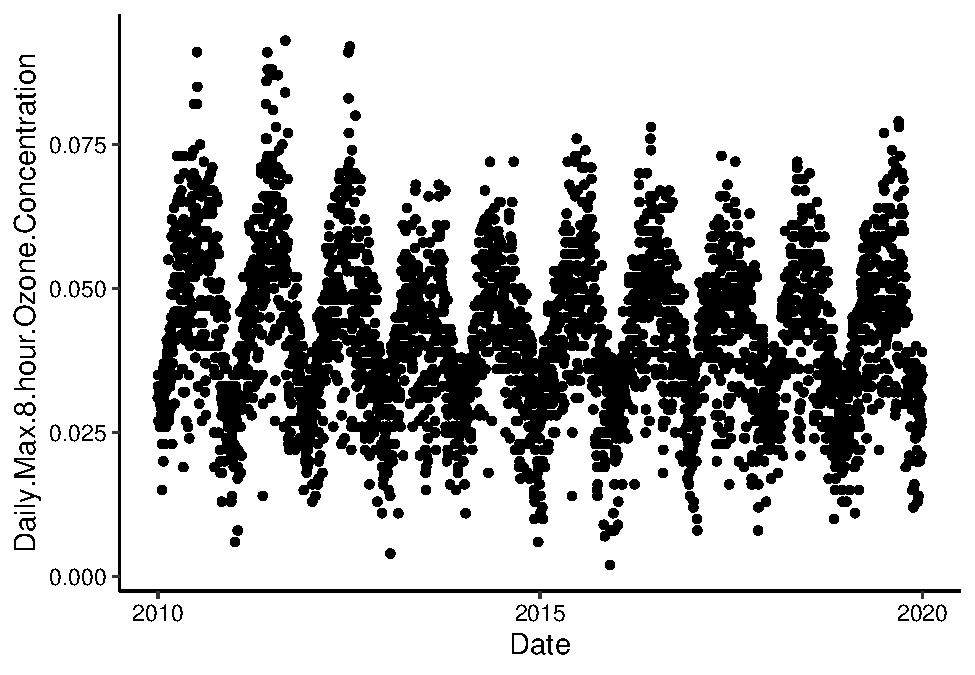
\includegraphics{A07_GLMs_Week2_files/figure-latex/unnamed-chunk-2-1.pdf}

\begin{enumerate}
\def\labelenumi{\arabic{enumi}.}
\setcounter{enumi}{4}
\tightlist
\item
  What is the final set of explanatory variables that predict
  temperature from your multiple regression? How much of the observed
  variance does this model explain?
\end{enumerate}

\begin{quote}
Answer: The final set of explanatory variables determined by our AIC
analysis are year, day number and depth (the same variables we started
with). The model explains 74.17\% of variance.
\end{quote}

\begin{enumerate}
\def\labelenumi{\arabic{enumi}.}
\setcounter{enumi}{5}
\tightlist
\item
  Run an interaction effects ANCOVA to predict temperature based on
  depth and lakename from the same wrangled dataset.
\end{enumerate}

\begin{Shaded}
\begin{Highlighting}[]
\CommentTok{#6}
\CommentTok{# want to see dif between main and interaction}
\CommentTok{# temp_ANCOVA_main <- lm(data = chem_phys_subset, temperature_C ~ depth + lakename)}
\NormalTok{temp_ANCOVA_interaction <-}\StringTok{ }\KeywordTok{lm}\NormalTok{(}\DataTypeTok{data =}\NormalTok{ chem_phys_subset, temperature_C }\OperatorTok{~}\StringTok{ }\NormalTok{depth }\OperatorTok{*}\StringTok{ }\NormalTok{lakename)}

\CommentTok{# summary(temp_ANCOVA_main) # 77.73% var explained}
\KeywordTok{summary}\NormalTok{(temp_ANCOVA_interaction) }\CommentTok{# 78.57% var explained}
\end{Highlighting}
\end{Shaded}

\begin{verbatim}
## 
## Call:
## lm(formula = temperature_C ~ depth * lakename, data = chem_phys_subset)
## 
## Residuals:
##     Min      1Q  Median      3Q     Max 
## -7.6455 -2.9133 -0.2879  2.7567 16.3606 
## 
## Coefficients:
##                                Estimate Std. Error t value Pr(>|t|)    
## (Intercept)                     22.9455     0.5861  39.147  < 2e-16 ***
## depth                           -2.5820     0.2411 -10.711  < 2e-16 ***
## lakenameCrampton Lake            2.2173     0.6804   3.259  0.00112 ** 
## lakenameEast Long Lake          -4.3884     0.6191  -7.089 1.45e-12 ***
## lakenameHummingbird Lake        -2.4126     0.8379  -2.879  0.00399 ** 
## lakenamePaul Lake                0.6105     0.5983   1.020  0.30754    
## lakenamePeter Lake               0.2998     0.5970   0.502  0.61552    
## lakenameTuesday Lake            -2.8932     0.6060  -4.774 1.83e-06 ***
## lakenameWard Lake                2.4180     0.8434   2.867  0.00415 ** 
## lakenameWest Long Lake          -2.4663     0.6168  -3.999 6.42e-05 ***
## depth:lakenameCrampton Lake      0.8058     0.2465   3.268  0.00109 ** 
## depth:lakenameEast Long Lake     0.9465     0.2433   3.891  0.00010 ***
## depth:lakenameHummingbird Lake  -0.6026     0.2919  -2.064  0.03903 *  
## depth:lakenamePaul Lake          0.4022     0.2421   1.662  0.09664 .  
## depth:lakenamePeter Lake         0.5799     0.2418   2.398  0.01649 *  
## depth:lakenameTuesday Lake       0.6605     0.2426   2.723  0.00648 ** 
## depth:lakenameWard Lake         -0.6930     0.2862  -2.421  0.01548 *  
## depth:lakenameWest Long Lake     0.8154     0.2431   3.354  0.00080 ***
## ---
## Signif. codes:  0 '***' 0.001 '**' 0.01 '*' 0.05 '.' 0.1 ' ' 1
## 
## Residual standard error: 3.471 on 9704 degrees of freedom
## Multiple R-squared:  0.7861, Adjusted R-squared:  0.7857 
## F-statistic:  2097 on 17 and 9704 DF,  p-value: < 2.2e-16
\end{verbatim}

\begin{enumerate}
\def\labelenumi{\arabic{enumi}.}
\setcounter{enumi}{6}
\tightlist
\item
  Is there a significant interaction between depth and lakename? How
  much variance in the temperature observations does this explain?
\end{enumerate}

\begin{quote}
Answer: Our results show that there is a significant interaction between
depth and lakename, meaning that depth varies significantly depending on
which lake we're sampling. Our interaction effects model explains
78.57\% of variance.
\end{quote}

\begin{enumerate}
\def\labelenumi{\arabic{enumi}.}
\setcounter{enumi}{7}
\tightlist
\item
  Create a graph that depicts temperature by depth, with a separate
  color for each lake. Add a geom\_smooth (method = ``lm'', se = FALSE)
  for each lake. Make your points 50 \% transparent. Adjust your y axis
  limits to go from 0 to 35 degrees. Clean up your graph to make it
  pretty.
\end{enumerate}

\begin{Shaded}
\begin{Highlighting}[]
\CommentTok{#8}
\NormalTok{temp_depth <-}\StringTok{ }
\StringTok{  }\KeywordTok{ggplot}\NormalTok{(chem_phys_subset, }\KeywordTok{aes}\NormalTok{(}\DataTypeTok{x =}\NormalTok{ depth, }\DataTypeTok{y =}\NormalTok{ temperature_C, }\DataTypeTok{color =}\NormalTok{ lakename)) }\OperatorTok{+}
\StringTok{  }\KeywordTok{geom_point}\NormalTok{(}\DataTypeTok{alpha =} \FloatTok{.5}\NormalTok{) }\OperatorTok{+}
\StringTok{  }\KeywordTok{ylim}\NormalTok{(}\DecValTok{0}\NormalTok{, }\DecValTok{35}\NormalTok{) }\OperatorTok{+}
\StringTok{  }\KeywordTok{labs}\NormalTok{(}\DataTypeTok{x =} \StringTok{"Depth (m)"}\NormalTok{, }\DataTypeTok{y =} \StringTok{"Temperature (˚C)"}\NormalTok{) }\OperatorTok{+}
\StringTok{  }\KeywordTok{geom_smooth}\NormalTok{(}\DataTypeTok{method =} \StringTok{'lm'}\NormalTok{, }\DataTypeTok{se =} \OtherTok{FALSE}\NormalTok{)}

\KeywordTok{print}\NormalTok{(temp_depth)}
\end{Highlighting}
\end{Shaded}

\begin{verbatim}
## Warning: Removed 73 rows containing missing values (geom_smooth).
\end{verbatim}

\begin{verbatim}
## Warning in grid.Call(C_textBounds, as.graphicsAnnot(x$label), x$x, x$y, :
## conversion failure on 'Temperature (˚C)' in 'mbcsToSbcs': dot substituted for
## <cb>
\end{verbatim}

\begin{verbatim}
## Warning in grid.Call(C_textBounds, as.graphicsAnnot(x$label), x$x, x$y, :
## conversion failure on 'Temperature (˚C)' in 'mbcsToSbcs': dot substituted for
## <9a>
\end{verbatim}

\begin{verbatim}
## Warning in grid.Call(C_textBounds, as.graphicsAnnot(x$label), x$x, x$y, :
## conversion failure on 'Temperature (˚C)' in 'mbcsToSbcs': dot substituted for
## <cb>
\end{verbatim}

\begin{verbatim}
## Warning in grid.Call(C_textBounds, as.graphicsAnnot(x$label), x$x, x$y, :
## conversion failure on 'Temperature (˚C)' in 'mbcsToSbcs': dot substituted for
## <9a>
\end{verbatim}

\begin{verbatim}
## Warning in grid.Call(C_textBounds, as.graphicsAnnot(x$label), x$x, x$y, :
## conversion failure on 'Temperature (˚C)' in 'mbcsToSbcs': dot substituted for
## <cb>
\end{verbatim}

\begin{verbatim}
## Warning in grid.Call(C_textBounds, as.graphicsAnnot(x$label), x$x, x$y, :
## conversion failure on 'Temperature (˚C)' in 'mbcsToSbcs': dot substituted for
## <9a>
\end{verbatim}

\begin{verbatim}
## Warning in grid.Call(C_textBounds, as.graphicsAnnot(x$label), x$x, x$y, :
## conversion failure on 'Temperature (˚C)' in 'mbcsToSbcs': dot substituted for
## <cb>
\end{verbatim}

\begin{verbatim}
## Warning in grid.Call(C_textBounds, as.graphicsAnnot(x$label), x$x, x$y, :
## conversion failure on 'Temperature (˚C)' in 'mbcsToSbcs': dot substituted for
## <9a>
\end{verbatim}

\begin{verbatim}
## Warning in grid.Call(C_textBounds, as.graphicsAnnot(x$label), x$x, x$y, :
## conversion failure on 'Temperature (˚C)' in 'mbcsToSbcs': dot substituted for
## <cb>
\end{verbatim}

\begin{verbatim}
## Warning in grid.Call(C_textBounds, as.graphicsAnnot(x$label), x$x, x$y, :
## conversion failure on 'Temperature (˚C)' in 'mbcsToSbcs': dot substituted for
## <9a>
\end{verbatim}

\begin{verbatim}
## Warning in grid.Call(C_textBounds, as.graphicsAnnot(x$label), x$x, x$y, :
## conversion failure on 'Temperature (˚C)' in 'mbcsToSbcs': dot substituted for
## <cb>
\end{verbatim}

\begin{verbatim}
## Warning in grid.Call(C_textBounds, as.graphicsAnnot(x$label), x$x, x$y, :
## conversion failure on 'Temperature (˚C)' in 'mbcsToSbcs': dot substituted for
## <9a>
\end{verbatim}

\begin{verbatim}
## Warning in grid.Call(C_textBounds, as.graphicsAnnot(x$label), x$x, x$y, :
## conversion failure on 'Temperature (˚C)' in 'mbcsToSbcs': dot substituted for
## <cb>
\end{verbatim}

\begin{verbatim}
## Warning in grid.Call(C_textBounds, as.graphicsAnnot(x$label), x$x, x$y, :
## conversion failure on 'Temperature (˚C)' in 'mbcsToSbcs': dot substituted for
## <9a>
\end{verbatim}

\begin{verbatim}
## Warning in grid.Call.graphics(C_text, as.graphicsAnnot(x$label), x$x, x$y, :
## conversion failure on 'Temperature (˚C)' in 'mbcsToSbcs': dot substituted for
## <cb>
\end{verbatim}

\begin{verbatim}
## Warning in grid.Call.graphics(C_text, as.graphicsAnnot(x$label), x$x, x$y, :
## conversion failure on 'Temperature (˚C)' in 'mbcsToSbcs': dot substituted for
## <9a>
\end{verbatim}

\includegraphics{A07_GLMs_Week2_files/figure-latex/unnamed-chunk-4-1.pdf}

\begin{enumerate}
\def\labelenumi{\arabic{enumi}.}
\setcounter{enumi}{8}
\tightlist
\item
  Run a mixed effects model to predict dry mass of litter. We already
  know that nlcdClass and functionalGroup have a significant
  interaction, so we will specify those two variables as fixed effects
  with an interaction. We also know that litter mass varies across plot
  ID, but we are less interested in the actual effect of the plot itself
  but rather in accounting for the variance among plots. Plot ID will be
  our random effect. \# litter dataset - looking to predict drymass of
  litter \# fixed effects = nlcdClass, functionalGroup (there is
  interaction between these) \# random effects = plotID
\end{enumerate}

\begin{enumerate}
\def\labelenumi{\alph{enumi}.}
\tightlist
\item
  Build and run a mixed effects model.
\item
  Check the difference between the marginal and conditional R2 of the
  model.
\end{enumerate}

\begin{Shaded}
\begin{Highlighting}[]
\NormalTok{LitterDrymass_mixed <-}\StringTok{ }
\StringTok{  }\KeywordTok{lme}\NormalTok{(}\DataTypeTok{data =}\NormalTok{ litter, dryMass }\OperatorTok{~}\StringTok{ }\NormalTok{nlcdClass }\OperatorTok{*}\StringTok{ }\NormalTok{functionalGroup, }\DataTypeTok{random =} \OperatorTok{~}\DecValTok{1}\OperatorTok{|}\NormalTok{plotID)}

\KeywordTok{summary}\NormalTok{(LitterDrymass_mixed) }\CommentTok{#}
\end{Highlighting}
\end{Shaded}

\begin{verbatim}
## Linear mixed-effects model fit by REML
##  Data: litter 
##        AIC      BIC    logLik
##   9038.575 9179.479 -4493.287
## 
## Random effects:
##  Formula: ~1 | plotID
##         (Intercept) Residual
## StdDev:   0.5899105 3.456817
## 
## Fixed effects: dryMass ~ nlcdClass * functionalGroup 
##                                                                Value Std.Error
## (Intercept)                                                 0.155492 0.4863580
## nlcdClassgrasslandHerbaceous                               -0.156004 0.7789816
## nlcdClassshrubScrub                                        -0.107080 0.6636775
## functionalGroupLeaves                                      -0.126008 0.5501061
## functionalGroupMixed                                        1.477797 0.6323043
## functionalGroupNeedles                                      7.284064 0.5313161
## functionalGroupOther                                       -0.048525 0.5500878
## functionalGroupSeeds                                       -0.058702 0.5501061
## functionalGroupTwigs/branches                               1.929441 0.5385556
## functionalGroupWoody material                               1.068772 0.5259330
## nlcdClassgrasslandHerbaceous:functionalGroupLeaves          0.181416 0.8847246
## nlcdClassshrubScrub:functionalGroupLeaves                   0.173857 0.7510320
## nlcdClassgrasslandHerbaceous:functionalGroupMixed          -0.467648 1.1201304
## nlcdClassshrubScrub:functionalGroupMixed                    0.633876 0.9217911
## nlcdClassgrasslandHerbaceous:functionalGroupNeedles        -2.118299 0.8705440
## nlcdClassshrubScrub:functionalGroupNeedles                 -2.909142 0.7347172
## nlcdClassgrasslandHerbaceous:functionalGroupOther           0.143603 0.8976715
## nlcdClassshrubScrub:functionalGroupOther                    0.104935 0.7528434
## nlcdClassgrasslandHerbaceous:functionalGroupSeeds           0.049290 0.8976827
## nlcdClassshrubScrub:functionalGroupSeeds                    0.076708 0.7547591
## nlcdClassgrasslandHerbaceous:functionalGroupTwigs/branches -0.986627 0.8850639
## nlcdClassshrubScrub:functionalGroupTwigs/branches          -1.503446 0.7409024
## nlcdClassgrasslandHerbaceous:functionalGroupWoody material -1.017803 0.8802289
## nlcdClassshrubScrub:functionalGroupWoody material          -0.979078 0.7317033
##                                                              DF   t-value
## (Intercept)                                                1659  0.319706
## nlcdClassgrasslandHerbaceous                                  9 -0.200266
## nlcdClassshrubScrub                                           9 -0.161343
## functionalGroupLeaves                                      1659 -0.229061
## functionalGroupMixed                                       1659  2.337160
## functionalGroupNeedles                                     1659 13.709474
## functionalGroupOther                                       1659 -0.088213
## functionalGroupSeeds                                       1659 -0.106711
## functionalGroupTwigs/branches                              1659  3.582622
## functionalGroupWoody material                              1659  2.032144
## nlcdClassgrasslandHerbaceous:functionalGroupLeaves         1659  0.205053
## nlcdClassshrubScrub:functionalGroupLeaves                  1659  0.231490
## nlcdClassgrasslandHerbaceous:functionalGroupMixed          1659 -0.417495
## nlcdClassshrubScrub:functionalGroupMixed                   1659  0.687657
## nlcdClassgrasslandHerbaceous:functionalGroupNeedles        1659 -2.433305
## nlcdClassshrubScrub:functionalGroupNeedles                 1659 -3.959540
## nlcdClassgrasslandHerbaceous:functionalGroupOther          1659  0.159972
## nlcdClassshrubScrub:functionalGroupOther                   1659  0.139385
## nlcdClassgrasslandHerbaceous:functionalGroupSeeds          1659  0.054908
## nlcdClassshrubScrub:functionalGroupSeeds                   1659  0.101632
## nlcdClassgrasslandHerbaceous:functionalGroupTwigs/branches 1659 -1.114752
## nlcdClassshrubScrub:functionalGroupTwigs/branches          1659 -2.029209
## nlcdClassgrasslandHerbaceous:functionalGroupWoody material 1659 -1.156293
## nlcdClassshrubScrub:functionalGroupWoody material          1659 -1.338081
##                                                            p-value
## (Intercept)                                                 0.7492
## nlcdClassgrasslandHerbaceous                                0.8457
## nlcdClassshrubScrub                                         0.8754
## functionalGroupLeaves                                       0.8188
## functionalGroupMixed                                        0.0195
## functionalGroupNeedles                                      0.0000
## functionalGroupOther                                        0.9297
## functionalGroupSeeds                                        0.9150
## functionalGroupTwigs/branches                               0.0003
## functionalGroupWoody material                               0.0423
## nlcdClassgrasslandHerbaceous:functionalGroupLeaves          0.8376
## nlcdClassshrubScrub:functionalGroupLeaves                   0.8170
## nlcdClassgrasslandHerbaceous:functionalGroupMixed           0.6764
## nlcdClassshrubScrub:functionalGroupMixed                    0.4918
## nlcdClassgrasslandHerbaceous:functionalGroupNeedles         0.0151
## nlcdClassshrubScrub:functionalGroupNeedles                  0.0001
## nlcdClassgrasslandHerbaceous:functionalGroupOther           0.8729
## nlcdClassshrubScrub:functionalGroupOther                    0.8892
## nlcdClassgrasslandHerbaceous:functionalGroupSeeds           0.9562
## nlcdClassshrubScrub:functionalGroupSeeds                    0.9191
## nlcdClassgrasslandHerbaceous:functionalGroupTwigs/branches  0.2651
## nlcdClassshrubScrub:functionalGroupTwigs/branches           0.0426
## nlcdClassgrasslandHerbaceous:functionalGroupWoody material  0.2477
## nlcdClassshrubScrub:functionalGroupWoody material           0.1811
##  Correlation: 
##                                                            (Intr) nlcdCH nlcdCS
## nlcdClassgrasslandHerbaceous                               -0.624              
## nlcdClassshrubScrub                                        -0.733  0.458       
## functionalGroupLeaves                                      -0.559  0.349  0.409
## functionalGroupMixed                                       -0.485  0.303  0.356
## functionalGroupNeedles                                     -0.579  0.361  0.424
## functionalGroupOther                                       -0.559  0.349  0.409
## functionalGroupSeeds                                       -0.559  0.349  0.409
## functionalGroupTwigs/branches                              -0.571  0.356  0.418
## functionalGroupWoody material                              -0.584  0.365  0.428
## nlcdClassgrasslandHerbaceous:functionalGroupLeaves          0.347 -0.586 -0.255
## nlcdClassshrubScrub:functionalGroupLeaves                   0.409 -0.255 -0.569
## nlcdClassgrasslandHerbaceous:functionalGroupMixed           0.274 -0.462 -0.201
## nlcdClassshrubScrub:functionalGroupMixed                    0.333 -0.208 -0.464
## nlcdClassgrasslandHerbaceous:functionalGroupNeedles         0.353 -0.595 -0.259
## nlcdClassshrubScrub:functionalGroupNeedles                  0.418 -0.261 -0.582
## nlcdClassgrasslandHerbaceous:functionalGroupOther           0.342 -0.577 -0.251
## nlcdClassshrubScrub:functionalGroupOther                    0.408 -0.255 -0.568
## nlcdClassgrasslandHerbaceous:functionalGroupSeeds           0.342 -0.577 -0.251
## nlcdClassshrubScrub:functionalGroupSeeds                    0.407 -0.254 -0.566
## nlcdClassgrasslandHerbaceous:functionalGroupTwigs/branches  0.347 -0.586 -0.254
## nlcdClassshrubScrub:functionalGroupTwigs/branches           0.415 -0.259 -0.577
## nlcdClassgrasslandHerbaceous:functionalGroupWoody material  0.349 -0.589 -0.256
## nlcdClassshrubScrub:functionalGroupWoody material           0.420 -0.262 -0.584
##                                                            fnctGL fnctGM fnctGN
## nlcdClassgrasslandHerbaceous                                                   
## nlcdClassshrubScrub                                                            
## functionalGroupLeaves                                                          
## functionalGroupMixed                                        0.429              
## functionalGroupNeedles                                      0.511  0.445       
## functionalGroupOther                                        0.494  0.430  0.511
## functionalGroupSeeds                                        0.494  0.429  0.511
## functionalGroupTwigs/branches                               0.504  0.439  0.522
## functionalGroupWoody material                               0.516  0.449  0.535
## nlcdClassgrasslandHerbaceous:functionalGroupLeaves         -0.622 -0.267 -0.318
## nlcdClassshrubScrub:functionalGroupLeaves                  -0.732 -0.314 -0.374
## nlcdClassgrasslandHerbaceous:functionalGroupMixed          -0.242 -0.564 -0.251
## nlcdClassshrubScrub:functionalGroupMixed                   -0.295 -0.686 -0.305
## nlcdClassgrasslandHerbaceous:functionalGroupNeedles        -0.312 -0.272 -0.610
## nlcdClassshrubScrub:functionalGroupNeedles                 -0.370 -0.322 -0.723
## nlcdClassgrasslandHerbaceous:functionalGroupOther          -0.303 -0.263 -0.313
## nlcdClassshrubScrub:functionalGroupOther                   -0.361 -0.314 -0.374
## nlcdClassgrasslandHerbaceous:functionalGroupSeeds          -0.303 -0.263 -0.313
## nlcdClassshrubScrub:functionalGroupSeeds                   -0.360 -0.313 -0.373
## nlcdClassgrasslandHerbaceous:functionalGroupTwigs/branches -0.307 -0.267 -0.318
## nlcdClassshrubScrub:functionalGroupTwigs/branches          -0.367 -0.319 -0.380
## nlcdClassgrasslandHerbaceous:functionalGroupWoody material -0.309 -0.268 -0.320
## nlcdClassshrubScrub:functionalGroupWoody material          -0.371 -0.322 -0.384
##                                                            fnctGO fnctGS fncGT/
## nlcdClassgrasslandHerbaceous                                                   
## nlcdClassshrubScrub                                                            
## functionalGroupLeaves                                                          
## functionalGroupMixed                                                           
## functionalGroupNeedles                                                         
## functionalGroupOther                                                           
## functionalGroupSeeds                                        0.494              
## functionalGroupTwigs/branches                               0.504  0.504       
## functionalGroupWoody material                               0.516  0.517  0.528
## nlcdClassgrasslandHerbaceous:functionalGroupLeaves         -0.307 -0.307 -0.314
## nlcdClassshrubScrub:functionalGroupLeaves                  -0.362 -0.362 -0.369
## nlcdClassgrasslandHerbaceous:functionalGroupMixed          -0.243 -0.242 -0.248
## nlcdClassshrubScrub:functionalGroupMixed                   -0.295 -0.294 -0.301
## nlcdClassgrasslandHerbaceous:functionalGroupNeedles        -0.312 -0.312 -0.319
## nlcdClassshrubScrub:functionalGroupNeedles                 -0.370 -0.370 -0.378
## nlcdClassgrasslandHerbaceous:functionalGroupOther          -0.613 -0.303 -0.309
## nlcdClassshrubScrub:functionalGroupOther                   -0.731 -0.361 -0.369
## nlcdClassgrasslandHerbaceous:functionalGroupSeeds          -0.303 -0.613 -0.309
## nlcdClassshrubScrub:functionalGroupSeeds                   -0.360 -0.729 -0.368
## nlcdClassgrasslandHerbaceous:functionalGroupTwigs/branches -0.307 -0.307 -0.608
## nlcdClassshrubScrub:functionalGroupTwigs/branches          -0.367 -0.367 -0.727
## nlcdClassgrasslandHerbaceous:functionalGroupWoody material -0.309 -0.309 -0.315
## nlcdClassshrubScrub:functionalGroupWoody material          -0.371 -0.371 -0.379
##                                                            fncGWm nCH:GL nCS:GL
## nlcdClassgrasslandHerbaceous                                                   
## nlcdClassshrubScrub                                                            
## functionalGroupLeaves                                                          
## functionalGroupMixed                                                           
## functionalGroupNeedles                                                         
## functionalGroupOther                                                           
## functionalGroupSeeds                                                           
## functionalGroupTwigs/branches                                                  
## functionalGroupWoody material                                                  
## nlcdClassgrasslandHerbaceous:functionalGroupLeaves         -0.321              
## nlcdClassshrubScrub:functionalGroupLeaves                  -0.378  0.455       
## nlcdClassgrasslandHerbaceous:functionalGroupMixed          -0.253  0.406  0.178
## nlcdClassshrubScrub:functionalGroupMixed                   -0.308  0.183  0.410
## nlcdClassgrasslandHerbaceous:functionalGroupNeedles        -0.326  0.524  0.229
## nlcdClassshrubScrub:functionalGroupNeedles                 -0.387  0.230  0.514
## nlcdClassgrasslandHerbaceous:functionalGroupOther          -0.316  0.508  0.222
## nlcdClassshrubScrub:functionalGroupOther                   -0.377  0.224  0.502
## nlcdClassgrasslandHerbaceous:functionalGroupSeeds          -0.317  0.508  0.222
## nlcdClassshrubScrub:functionalGroupSeeds                   -0.376  0.224  0.500
## nlcdClassgrasslandHerbaceous:functionalGroupTwigs/branches -0.321  0.515  0.225
## nlcdClassshrubScrub:functionalGroupTwigs/branches          -0.384  0.228  0.510
## nlcdClassgrasslandHerbaceous:functionalGroupWoody material -0.597  0.518  0.226
## nlcdClassshrubScrub:functionalGroupWoody material          -0.719  0.231  0.516
##                                                            nCH:GM nCS:GM nCH:GN
## nlcdClassgrasslandHerbaceous                                                   
## nlcdClassshrubScrub                                                            
## functionalGroupLeaves                                                          
## functionalGroupMixed                                                           
## functionalGroupNeedles                                                         
## functionalGroupOther                                                           
## functionalGroupSeeds                                                           
## functionalGroupTwigs/branches                                                  
## functionalGroupWoody material                                                  
## nlcdClassgrasslandHerbaceous:functionalGroupLeaves                             
## nlcdClassshrubScrub:functionalGroupLeaves                                      
## nlcdClassgrasslandHerbaceous:functionalGroupMixed                              
## nlcdClassshrubScrub:functionalGroupMixed                    0.387              
## nlcdClassgrasslandHerbaceous:functionalGroupNeedles         0.414  0.186       
## nlcdClassshrubScrub:functionalGroupNeedles                  0.182  0.419  0.441
## nlcdClassgrasslandHerbaceous:functionalGroupOther           0.401  0.181  0.517
## nlcdClassshrubScrub:functionalGroupOther                    0.177  0.409  0.228
## nlcdClassgrasslandHerbaceous:functionalGroupSeeds           0.402  0.180  0.517
## nlcdClassshrubScrub:functionalGroupSeeds                    0.177  0.408  0.227
## nlcdClassgrasslandHerbaceous:functionalGroupTwigs/branches  0.407  0.183  0.524
## nlcdClassshrubScrub:functionalGroupTwigs/branches           0.180  0.416  0.232
## nlcdClassgrasslandHerbaceous:functionalGroupWoody material  0.409  0.184  0.527
## nlcdClassshrubScrub:functionalGroupWoody material           0.182  0.420  0.235
##                                                            nCS:GN nCH:GO nCS:GO
## nlcdClassgrasslandHerbaceous                                                   
## nlcdClassshrubScrub                                                            
## functionalGroupLeaves                                                          
## functionalGroupMixed                                                           
## functionalGroupNeedles                                                         
## functionalGroupOther                                                           
## functionalGroupSeeds                                                           
## functionalGroupTwigs/branches                                                  
## functionalGroupWoody material                                                  
## nlcdClassgrasslandHerbaceous:functionalGroupLeaves                             
## nlcdClassshrubScrub:functionalGroupLeaves                                      
## nlcdClassgrasslandHerbaceous:functionalGroupMixed                              
## nlcdClassshrubScrub:functionalGroupMixed                                       
## nlcdClassgrasslandHerbaceous:functionalGroupNeedles                            
## nlcdClassshrubScrub:functionalGroupNeedles                                     
## nlcdClassgrasslandHerbaceous:functionalGroupOther           0.227              
## nlcdClassshrubScrub:functionalGroupOther                    0.513  0.448       
## nlcdClassgrasslandHerbaceous:functionalGroupSeeds           0.227  0.501  0.221
## nlcdClassshrubScrub:functionalGroupSeeds                    0.512  0.221  0.499
## nlcdClassgrasslandHerbaceous:functionalGroupTwigs/branches  0.230  0.508  0.224
## nlcdClassshrubScrub:functionalGroupTwigs/branches           0.521  0.225  0.509
## nlcdClassgrasslandHerbaceous:functionalGroupWoody material  0.231  0.511  0.225
## nlcdClassshrubScrub:functionalGroupWoody material           0.528  0.227  0.515
##                                                            nCH:GS nCS:GS nCH:GT
## nlcdClassgrasslandHerbaceous                                                   
## nlcdClassshrubScrub                                                            
## functionalGroupLeaves                                                          
## functionalGroupMixed                                                           
## functionalGroupNeedles                                                         
## functionalGroupOther                                                           
## functionalGroupSeeds                                                           
## functionalGroupTwigs/branches                                                  
## functionalGroupWoody material                                                  
## nlcdClassgrasslandHerbaceous:functionalGroupLeaves                             
## nlcdClassshrubScrub:functionalGroupLeaves                                      
## nlcdClassgrasslandHerbaceous:functionalGroupMixed                              
## nlcdClassshrubScrub:functionalGroupMixed                                       
## nlcdClassgrasslandHerbaceous:functionalGroupNeedles                            
## nlcdClassshrubScrub:functionalGroupNeedles                                     
## nlcdClassgrasslandHerbaceous:functionalGroupOther                              
## nlcdClassshrubScrub:functionalGroupOther                                       
## nlcdClassgrasslandHerbaceous:functionalGroupSeeds                              
## nlcdClassshrubScrub:functionalGroupSeeds                    0.447              
## nlcdClassgrasslandHerbaceous:functionalGroupTwigs/branches  0.508  0.224       
## nlcdClassshrubScrub:functionalGroupTwigs/branches           0.225  0.507  0.442
## nlcdClassgrasslandHerbaceous:functionalGroupWoody material  0.511  0.225  0.518
## nlcdClassshrubScrub:functionalGroupWoody material           0.228  0.514  0.231
##                                                            nCS:GT nCH:Gm
## nlcdClassgrasslandHerbaceous                                            
## nlcdClassshrubScrub                                                     
## functionalGroupLeaves                                                   
## functionalGroupMixed                                                    
## functionalGroupNeedles                                                  
## functionalGroupOther                                                    
## functionalGroupSeeds                                                    
## functionalGroupTwigs/branches                                           
## functionalGroupWoody material                                           
## nlcdClassgrasslandHerbaceous:functionalGroupLeaves                      
## nlcdClassshrubScrub:functionalGroupLeaves                               
## nlcdClassgrasslandHerbaceous:functionalGroupMixed                       
## nlcdClassshrubScrub:functionalGroupMixed                                
## nlcdClassgrasslandHerbaceous:functionalGroupNeedles                     
## nlcdClassshrubScrub:functionalGroupNeedles                              
## nlcdClassgrasslandHerbaceous:functionalGroupOther                       
## nlcdClassshrubScrub:functionalGroupOther                                
## nlcdClassgrasslandHerbaceous:functionalGroupSeeds                       
## nlcdClassshrubScrub:functionalGroupSeeds                                
## nlcdClassgrasslandHerbaceous:functionalGroupTwigs/branches              
## nlcdClassshrubScrub:functionalGroupTwigs/branches                       
## nlcdClassgrasslandHerbaceous:functionalGroupWoody material  0.229       
## nlcdClassshrubScrub:functionalGroupWoody material           0.523  0.429
## 
## Standardized Within-Group Residuals:
##         Min          Q1         Med          Q3         Max 
## -1.96496855 -0.23842984 -0.01535880  0.09027291 14.27434811 
## 
## Number of Observations: 1692
## Number of Groups: 12
\end{verbatim}

\begin{Shaded}
\begin{Highlighting}[]
\NormalTok{rsq <-}\StringTok{ }\KeywordTok{rsquared}\NormalTok{(LitterDrymass_mixed)}
\NormalTok{rsq}
\end{Highlighting}
\end{Shaded}

\begin{verbatim}
##   Response   family     link method  Marginal Conditional
## 1  dryMass gaussian identity   none 0.2465822   0.2679023
\end{verbatim}

\begin{Shaded}
\begin{Highlighting}[]
\NormalTok{R2_diff <-}\StringTok{ }\KeywordTok{as.numeric}\NormalTok{(rsq}\OperatorTok{$}\NormalTok{Marginal }\OperatorTok{-}\StringTok{ }\NormalTok{rsq}\OperatorTok{$}\NormalTok{Conditional)}
\NormalTok{R2_diff}
\end{Highlighting}
\end{Shaded}

\begin{verbatim}
## [1] -0.02132006
\end{verbatim}

\begin{enumerate}
\def\labelenumi{\alph{enumi}.}
\setcounter{enumi}{1}
\tightlist
\item
  continued\ldots{} How much more variance is explained by adding the
  random effect to the model?
\end{enumerate}

\begin{quote}
Answer: \textasciitilde{}2.13 \%
\end{quote}

\begin{enumerate}
\def\labelenumi{\alph{enumi}.}
\setcounter{enumi}{2}
\tightlist
\item
  Run the same model without the random effect.
\item
  Run an anova on the two tests.
\end{enumerate}

\begin{Shaded}
\begin{Highlighting}[]
\NormalTok{LitterDrymass_fixed <-}\StringTok{ }
\StringTok{  }\KeywordTok{lm}\NormalTok{(}\DataTypeTok{data =}\NormalTok{ litter, dryMass }\OperatorTok{~}\StringTok{ }\NormalTok{nlcdClass }\OperatorTok{*}\StringTok{ }\NormalTok{functionalGroup) }
\CommentTok{# we were told that the two variables have interaction, thus we multiply}


\KeywordTok{summary}\NormalTok{(LitterDrymass_fixed)}
\end{Highlighting}
\end{Shaded}

\begin{verbatim}
## 
## Call:
## lm(formula = dryMass ~ nlcdClass * functionalGroup, data = litter)
## 
## Residuals:
##    Min     1Q Median     3Q    Max 
## -6.612 -0.480 -0.058 -0.005 49.051 
## 
## Coefficients:
##                                                            Estimate Std. Error
## (Intercept)                                                 0.11963    0.39070
## nlcdClassgrasslandHerbaceous                               -0.11420    0.64223
## nlcdClassshrubScrub                                        -0.10412    0.53838
## functionalGroupLeaves                                      -0.10360    0.55606
## functionalGroupMixed                                        1.50475    0.63800
## functionalGroupNeedles                                      7.31226    0.53696
## functionalGroupOther                                       -0.03482    0.55606
## functionalGroupSeeds                                       -0.04616    0.55606
## functionalGroupTwigs/branches                               1.95967    0.54434
## functionalGroupWoody material                               1.08431    0.53156
## nlcdClassgrasslandHerbaceous:functionalGroupLeaves          0.12865    0.89410
## nlcdClassshrubScrub:functionalGroupLeaves                   0.14703    0.75915
## nlcdClassgrasslandHerbaceous:functionalGroupMixed          -0.38118    1.13024
## nlcdClassshrubScrub:functionalGroupMixed                    0.74593    0.93038
## nlcdClassgrasslandHerbaceous:functionalGroupNeedles        -2.13880    0.87993
## nlcdClassshrubScrub:functionalGroupNeedles                 -2.92148    0.74258
## nlcdClassgrasslandHerbaceous:functionalGroupOther           0.12606    0.90743
## nlcdClassshrubScrub:functionalGroupOther                    0.08589    0.76101
## nlcdClassgrasslandHerbaceous:functionalGroupSeeds           0.04615    0.90743
## nlcdClassshrubScrub:functionalGroupSeeds                    0.05944    0.76295
## nlcdClassgrasslandHerbaceous:functionalGroupTwigs/branches -1.01519    0.89462
## nlcdClassshrubScrub:functionalGroupTwigs/branches          -1.49559    0.74881
## nlcdClassgrasslandHerbaceous:functionalGroupWoody material -1.04086    0.88971
## nlcdClassshrubScrub:functionalGroupWoody material          -0.97185    0.73957
##                                                            t value Pr(>|t|)    
## (Intercept)                                                  0.306 0.759502    
## nlcdClassgrasslandHerbaceous                                -0.178 0.858888    
## nlcdClassshrubScrub                                         -0.193 0.846673    
## functionalGroupLeaves                                       -0.186 0.852224    
## functionalGroupMixed                                         2.359 0.018462 *  
## functionalGroupNeedles                                      13.618  < 2e-16 ***
## functionalGroupOther                                        -0.063 0.950081    
## functionalGroupSeeds                                        -0.083 0.933846    
## functionalGroupTwigs/branches                                3.600 0.000327 ***
## functionalGroupWoody material                                2.040 0.041519 *  
## nlcdClassgrasslandHerbaceous:functionalGroupLeaves           0.144 0.885611    
## nlcdClassshrubScrub:functionalGroupLeaves                    0.194 0.846453    
## nlcdClassgrasslandHerbaceous:functionalGroupMixed           -0.337 0.735969    
## nlcdClassshrubScrub:functionalGroupMixed                     0.802 0.422814    
## nlcdClassgrasslandHerbaceous:functionalGroupNeedles         -2.431 0.015177 *  
## nlcdClassshrubScrub:functionalGroupNeedles                  -3.934 8.69e-05 ***
## nlcdClassgrasslandHerbaceous:functionalGroupOther            0.139 0.889531    
## nlcdClassshrubScrub:functionalGroupOther                     0.113 0.910155    
## nlcdClassgrasslandHerbaceous:functionalGroupSeeds            0.051 0.959441    
## nlcdClassshrubScrub:functionalGroupSeeds                     0.078 0.937915    
## nlcdClassgrasslandHerbaceous:functionalGroupTwigs/branches  -1.135 0.256634    
## nlcdClassshrubScrub:functionalGroupTwigs/branches           -1.997 0.045956 *  
## nlcdClassgrasslandHerbaceous:functionalGroupWoody material  -1.170 0.242213    
## nlcdClassshrubScrub:functionalGroupWoody material           -1.314 0.189001    
## ---
## Signif. codes:  0 '***' 0.001 '**' 0.01 '*' 0.05 '.' 0.1 ' ' 1
## 
## Residual standard error: 3.494 on 1668 degrees of freedom
## Multiple R-squared:  0.2516, Adjusted R-squared:  0.2413 
## F-statistic: 24.38 on 23 and 1668 DF,  p-value: < 2.2e-16
\end{verbatim}

\begin{Shaded}
\begin{Highlighting}[]
\KeywordTok{summary}\NormalTok{(LitterDrymass_mixed)}
\end{Highlighting}
\end{Shaded}

\begin{verbatim}
## Linear mixed-effects model fit by REML
##  Data: litter 
##        AIC      BIC    logLik
##   9038.575 9179.479 -4493.287
## 
## Random effects:
##  Formula: ~1 | plotID
##         (Intercept) Residual
## StdDev:   0.5899105 3.456817
## 
## Fixed effects: dryMass ~ nlcdClass * functionalGroup 
##                                                                Value Std.Error
## (Intercept)                                                 0.155492 0.4863580
## nlcdClassgrasslandHerbaceous                               -0.156004 0.7789816
## nlcdClassshrubScrub                                        -0.107080 0.6636775
## functionalGroupLeaves                                      -0.126008 0.5501061
## functionalGroupMixed                                        1.477797 0.6323043
## functionalGroupNeedles                                      7.284064 0.5313161
## functionalGroupOther                                       -0.048525 0.5500878
## functionalGroupSeeds                                       -0.058702 0.5501061
## functionalGroupTwigs/branches                               1.929441 0.5385556
## functionalGroupWoody material                               1.068772 0.5259330
## nlcdClassgrasslandHerbaceous:functionalGroupLeaves          0.181416 0.8847246
## nlcdClassshrubScrub:functionalGroupLeaves                   0.173857 0.7510320
## nlcdClassgrasslandHerbaceous:functionalGroupMixed          -0.467648 1.1201304
## nlcdClassshrubScrub:functionalGroupMixed                    0.633876 0.9217911
## nlcdClassgrasslandHerbaceous:functionalGroupNeedles        -2.118299 0.8705440
## nlcdClassshrubScrub:functionalGroupNeedles                 -2.909142 0.7347172
## nlcdClassgrasslandHerbaceous:functionalGroupOther           0.143603 0.8976715
## nlcdClassshrubScrub:functionalGroupOther                    0.104935 0.7528434
## nlcdClassgrasslandHerbaceous:functionalGroupSeeds           0.049290 0.8976827
## nlcdClassshrubScrub:functionalGroupSeeds                    0.076708 0.7547591
## nlcdClassgrasslandHerbaceous:functionalGroupTwigs/branches -0.986627 0.8850639
## nlcdClassshrubScrub:functionalGroupTwigs/branches          -1.503446 0.7409024
## nlcdClassgrasslandHerbaceous:functionalGroupWoody material -1.017803 0.8802289
## nlcdClassshrubScrub:functionalGroupWoody material          -0.979078 0.7317033
##                                                              DF   t-value
## (Intercept)                                                1659  0.319706
## nlcdClassgrasslandHerbaceous                                  9 -0.200266
## nlcdClassshrubScrub                                           9 -0.161343
## functionalGroupLeaves                                      1659 -0.229061
## functionalGroupMixed                                       1659  2.337160
## functionalGroupNeedles                                     1659 13.709474
## functionalGroupOther                                       1659 -0.088213
## functionalGroupSeeds                                       1659 -0.106711
## functionalGroupTwigs/branches                              1659  3.582622
## functionalGroupWoody material                              1659  2.032144
## nlcdClassgrasslandHerbaceous:functionalGroupLeaves         1659  0.205053
## nlcdClassshrubScrub:functionalGroupLeaves                  1659  0.231490
## nlcdClassgrasslandHerbaceous:functionalGroupMixed          1659 -0.417495
## nlcdClassshrubScrub:functionalGroupMixed                   1659  0.687657
## nlcdClassgrasslandHerbaceous:functionalGroupNeedles        1659 -2.433305
## nlcdClassshrubScrub:functionalGroupNeedles                 1659 -3.959540
## nlcdClassgrasslandHerbaceous:functionalGroupOther          1659  0.159972
## nlcdClassshrubScrub:functionalGroupOther                   1659  0.139385
## nlcdClassgrasslandHerbaceous:functionalGroupSeeds          1659  0.054908
## nlcdClassshrubScrub:functionalGroupSeeds                   1659  0.101632
## nlcdClassgrasslandHerbaceous:functionalGroupTwigs/branches 1659 -1.114752
## nlcdClassshrubScrub:functionalGroupTwigs/branches          1659 -2.029209
## nlcdClassgrasslandHerbaceous:functionalGroupWoody material 1659 -1.156293
## nlcdClassshrubScrub:functionalGroupWoody material          1659 -1.338081
##                                                            p-value
## (Intercept)                                                 0.7492
## nlcdClassgrasslandHerbaceous                                0.8457
## nlcdClassshrubScrub                                         0.8754
## functionalGroupLeaves                                       0.8188
## functionalGroupMixed                                        0.0195
## functionalGroupNeedles                                      0.0000
## functionalGroupOther                                        0.9297
## functionalGroupSeeds                                        0.9150
## functionalGroupTwigs/branches                               0.0003
## functionalGroupWoody material                               0.0423
## nlcdClassgrasslandHerbaceous:functionalGroupLeaves          0.8376
## nlcdClassshrubScrub:functionalGroupLeaves                   0.8170
## nlcdClassgrasslandHerbaceous:functionalGroupMixed           0.6764
## nlcdClassshrubScrub:functionalGroupMixed                    0.4918
## nlcdClassgrasslandHerbaceous:functionalGroupNeedles         0.0151
## nlcdClassshrubScrub:functionalGroupNeedles                  0.0001
## nlcdClassgrasslandHerbaceous:functionalGroupOther           0.8729
## nlcdClassshrubScrub:functionalGroupOther                    0.8892
## nlcdClassgrasslandHerbaceous:functionalGroupSeeds           0.9562
## nlcdClassshrubScrub:functionalGroupSeeds                    0.9191
## nlcdClassgrasslandHerbaceous:functionalGroupTwigs/branches  0.2651
## nlcdClassshrubScrub:functionalGroupTwigs/branches           0.0426
## nlcdClassgrasslandHerbaceous:functionalGroupWoody material  0.2477
## nlcdClassshrubScrub:functionalGroupWoody material           0.1811
##  Correlation: 
##                                                            (Intr) nlcdCH nlcdCS
## nlcdClassgrasslandHerbaceous                               -0.624              
## nlcdClassshrubScrub                                        -0.733  0.458       
## functionalGroupLeaves                                      -0.559  0.349  0.409
## functionalGroupMixed                                       -0.485  0.303  0.356
## functionalGroupNeedles                                     -0.579  0.361  0.424
## functionalGroupOther                                       -0.559  0.349  0.409
## functionalGroupSeeds                                       -0.559  0.349  0.409
## functionalGroupTwigs/branches                              -0.571  0.356  0.418
## functionalGroupWoody material                              -0.584  0.365  0.428
## nlcdClassgrasslandHerbaceous:functionalGroupLeaves          0.347 -0.586 -0.255
## nlcdClassshrubScrub:functionalGroupLeaves                   0.409 -0.255 -0.569
## nlcdClassgrasslandHerbaceous:functionalGroupMixed           0.274 -0.462 -0.201
## nlcdClassshrubScrub:functionalGroupMixed                    0.333 -0.208 -0.464
## nlcdClassgrasslandHerbaceous:functionalGroupNeedles         0.353 -0.595 -0.259
## nlcdClassshrubScrub:functionalGroupNeedles                  0.418 -0.261 -0.582
## nlcdClassgrasslandHerbaceous:functionalGroupOther           0.342 -0.577 -0.251
## nlcdClassshrubScrub:functionalGroupOther                    0.408 -0.255 -0.568
## nlcdClassgrasslandHerbaceous:functionalGroupSeeds           0.342 -0.577 -0.251
## nlcdClassshrubScrub:functionalGroupSeeds                    0.407 -0.254 -0.566
## nlcdClassgrasslandHerbaceous:functionalGroupTwigs/branches  0.347 -0.586 -0.254
## nlcdClassshrubScrub:functionalGroupTwigs/branches           0.415 -0.259 -0.577
## nlcdClassgrasslandHerbaceous:functionalGroupWoody material  0.349 -0.589 -0.256
## nlcdClassshrubScrub:functionalGroupWoody material           0.420 -0.262 -0.584
##                                                            fnctGL fnctGM fnctGN
## nlcdClassgrasslandHerbaceous                                                   
## nlcdClassshrubScrub                                                            
## functionalGroupLeaves                                                          
## functionalGroupMixed                                        0.429              
## functionalGroupNeedles                                      0.511  0.445       
## functionalGroupOther                                        0.494  0.430  0.511
## functionalGroupSeeds                                        0.494  0.429  0.511
## functionalGroupTwigs/branches                               0.504  0.439  0.522
## functionalGroupWoody material                               0.516  0.449  0.535
## nlcdClassgrasslandHerbaceous:functionalGroupLeaves         -0.622 -0.267 -0.318
## nlcdClassshrubScrub:functionalGroupLeaves                  -0.732 -0.314 -0.374
## nlcdClassgrasslandHerbaceous:functionalGroupMixed          -0.242 -0.564 -0.251
## nlcdClassshrubScrub:functionalGroupMixed                   -0.295 -0.686 -0.305
## nlcdClassgrasslandHerbaceous:functionalGroupNeedles        -0.312 -0.272 -0.610
## nlcdClassshrubScrub:functionalGroupNeedles                 -0.370 -0.322 -0.723
## nlcdClassgrasslandHerbaceous:functionalGroupOther          -0.303 -0.263 -0.313
## nlcdClassshrubScrub:functionalGroupOther                   -0.361 -0.314 -0.374
## nlcdClassgrasslandHerbaceous:functionalGroupSeeds          -0.303 -0.263 -0.313
## nlcdClassshrubScrub:functionalGroupSeeds                   -0.360 -0.313 -0.373
## nlcdClassgrasslandHerbaceous:functionalGroupTwigs/branches -0.307 -0.267 -0.318
## nlcdClassshrubScrub:functionalGroupTwigs/branches          -0.367 -0.319 -0.380
## nlcdClassgrasslandHerbaceous:functionalGroupWoody material -0.309 -0.268 -0.320
## nlcdClassshrubScrub:functionalGroupWoody material          -0.371 -0.322 -0.384
##                                                            fnctGO fnctGS fncGT/
## nlcdClassgrasslandHerbaceous                                                   
## nlcdClassshrubScrub                                                            
## functionalGroupLeaves                                                          
## functionalGroupMixed                                                           
## functionalGroupNeedles                                                         
## functionalGroupOther                                                           
## functionalGroupSeeds                                        0.494              
## functionalGroupTwigs/branches                               0.504  0.504       
## functionalGroupWoody material                               0.516  0.517  0.528
## nlcdClassgrasslandHerbaceous:functionalGroupLeaves         -0.307 -0.307 -0.314
## nlcdClassshrubScrub:functionalGroupLeaves                  -0.362 -0.362 -0.369
## nlcdClassgrasslandHerbaceous:functionalGroupMixed          -0.243 -0.242 -0.248
## nlcdClassshrubScrub:functionalGroupMixed                   -0.295 -0.294 -0.301
## nlcdClassgrasslandHerbaceous:functionalGroupNeedles        -0.312 -0.312 -0.319
## nlcdClassshrubScrub:functionalGroupNeedles                 -0.370 -0.370 -0.378
## nlcdClassgrasslandHerbaceous:functionalGroupOther          -0.613 -0.303 -0.309
## nlcdClassshrubScrub:functionalGroupOther                   -0.731 -0.361 -0.369
## nlcdClassgrasslandHerbaceous:functionalGroupSeeds          -0.303 -0.613 -0.309
## nlcdClassshrubScrub:functionalGroupSeeds                   -0.360 -0.729 -0.368
## nlcdClassgrasslandHerbaceous:functionalGroupTwigs/branches -0.307 -0.307 -0.608
## nlcdClassshrubScrub:functionalGroupTwigs/branches          -0.367 -0.367 -0.727
## nlcdClassgrasslandHerbaceous:functionalGroupWoody material -0.309 -0.309 -0.315
## nlcdClassshrubScrub:functionalGroupWoody material          -0.371 -0.371 -0.379
##                                                            fncGWm nCH:GL nCS:GL
## nlcdClassgrasslandHerbaceous                                                   
## nlcdClassshrubScrub                                                            
## functionalGroupLeaves                                                          
## functionalGroupMixed                                                           
## functionalGroupNeedles                                                         
## functionalGroupOther                                                           
## functionalGroupSeeds                                                           
## functionalGroupTwigs/branches                                                  
## functionalGroupWoody material                                                  
## nlcdClassgrasslandHerbaceous:functionalGroupLeaves         -0.321              
## nlcdClassshrubScrub:functionalGroupLeaves                  -0.378  0.455       
## nlcdClassgrasslandHerbaceous:functionalGroupMixed          -0.253  0.406  0.178
## nlcdClassshrubScrub:functionalGroupMixed                   -0.308  0.183  0.410
## nlcdClassgrasslandHerbaceous:functionalGroupNeedles        -0.326  0.524  0.229
## nlcdClassshrubScrub:functionalGroupNeedles                 -0.387  0.230  0.514
## nlcdClassgrasslandHerbaceous:functionalGroupOther          -0.316  0.508  0.222
## nlcdClassshrubScrub:functionalGroupOther                   -0.377  0.224  0.502
## nlcdClassgrasslandHerbaceous:functionalGroupSeeds          -0.317  0.508  0.222
## nlcdClassshrubScrub:functionalGroupSeeds                   -0.376  0.224  0.500
## nlcdClassgrasslandHerbaceous:functionalGroupTwigs/branches -0.321  0.515  0.225
## nlcdClassshrubScrub:functionalGroupTwigs/branches          -0.384  0.228  0.510
## nlcdClassgrasslandHerbaceous:functionalGroupWoody material -0.597  0.518  0.226
## nlcdClassshrubScrub:functionalGroupWoody material          -0.719  0.231  0.516
##                                                            nCH:GM nCS:GM nCH:GN
## nlcdClassgrasslandHerbaceous                                                   
## nlcdClassshrubScrub                                                            
## functionalGroupLeaves                                                          
## functionalGroupMixed                                                           
## functionalGroupNeedles                                                         
## functionalGroupOther                                                           
## functionalGroupSeeds                                                           
## functionalGroupTwigs/branches                                                  
## functionalGroupWoody material                                                  
## nlcdClassgrasslandHerbaceous:functionalGroupLeaves                             
## nlcdClassshrubScrub:functionalGroupLeaves                                      
## nlcdClassgrasslandHerbaceous:functionalGroupMixed                              
## nlcdClassshrubScrub:functionalGroupMixed                    0.387              
## nlcdClassgrasslandHerbaceous:functionalGroupNeedles         0.414  0.186       
## nlcdClassshrubScrub:functionalGroupNeedles                  0.182  0.419  0.441
## nlcdClassgrasslandHerbaceous:functionalGroupOther           0.401  0.181  0.517
## nlcdClassshrubScrub:functionalGroupOther                    0.177  0.409  0.228
## nlcdClassgrasslandHerbaceous:functionalGroupSeeds           0.402  0.180  0.517
## nlcdClassshrubScrub:functionalGroupSeeds                    0.177  0.408  0.227
## nlcdClassgrasslandHerbaceous:functionalGroupTwigs/branches  0.407  0.183  0.524
## nlcdClassshrubScrub:functionalGroupTwigs/branches           0.180  0.416  0.232
## nlcdClassgrasslandHerbaceous:functionalGroupWoody material  0.409  0.184  0.527
## nlcdClassshrubScrub:functionalGroupWoody material           0.182  0.420  0.235
##                                                            nCS:GN nCH:GO nCS:GO
## nlcdClassgrasslandHerbaceous                                                   
## nlcdClassshrubScrub                                                            
## functionalGroupLeaves                                                          
## functionalGroupMixed                                                           
## functionalGroupNeedles                                                         
## functionalGroupOther                                                           
## functionalGroupSeeds                                                           
## functionalGroupTwigs/branches                                                  
## functionalGroupWoody material                                                  
## nlcdClassgrasslandHerbaceous:functionalGroupLeaves                             
## nlcdClassshrubScrub:functionalGroupLeaves                                      
## nlcdClassgrasslandHerbaceous:functionalGroupMixed                              
## nlcdClassshrubScrub:functionalGroupMixed                                       
## nlcdClassgrasslandHerbaceous:functionalGroupNeedles                            
## nlcdClassshrubScrub:functionalGroupNeedles                                     
## nlcdClassgrasslandHerbaceous:functionalGroupOther           0.227              
## nlcdClassshrubScrub:functionalGroupOther                    0.513  0.448       
## nlcdClassgrasslandHerbaceous:functionalGroupSeeds           0.227  0.501  0.221
## nlcdClassshrubScrub:functionalGroupSeeds                    0.512  0.221  0.499
## nlcdClassgrasslandHerbaceous:functionalGroupTwigs/branches  0.230  0.508  0.224
## nlcdClassshrubScrub:functionalGroupTwigs/branches           0.521  0.225  0.509
## nlcdClassgrasslandHerbaceous:functionalGroupWoody material  0.231  0.511  0.225
## nlcdClassshrubScrub:functionalGroupWoody material           0.528  0.227  0.515
##                                                            nCH:GS nCS:GS nCH:GT
## nlcdClassgrasslandHerbaceous                                                   
## nlcdClassshrubScrub                                                            
## functionalGroupLeaves                                                          
## functionalGroupMixed                                                           
## functionalGroupNeedles                                                         
## functionalGroupOther                                                           
## functionalGroupSeeds                                                           
## functionalGroupTwigs/branches                                                  
## functionalGroupWoody material                                                  
## nlcdClassgrasslandHerbaceous:functionalGroupLeaves                             
## nlcdClassshrubScrub:functionalGroupLeaves                                      
## nlcdClassgrasslandHerbaceous:functionalGroupMixed                              
## nlcdClassshrubScrub:functionalGroupMixed                                       
## nlcdClassgrasslandHerbaceous:functionalGroupNeedles                            
## nlcdClassshrubScrub:functionalGroupNeedles                                     
## nlcdClassgrasslandHerbaceous:functionalGroupOther                              
## nlcdClassshrubScrub:functionalGroupOther                                       
## nlcdClassgrasslandHerbaceous:functionalGroupSeeds                              
## nlcdClassshrubScrub:functionalGroupSeeds                    0.447              
## nlcdClassgrasslandHerbaceous:functionalGroupTwigs/branches  0.508  0.224       
## nlcdClassshrubScrub:functionalGroupTwigs/branches           0.225  0.507  0.442
## nlcdClassgrasslandHerbaceous:functionalGroupWoody material  0.511  0.225  0.518
## nlcdClassshrubScrub:functionalGroupWoody material           0.228  0.514  0.231
##                                                            nCS:GT nCH:Gm
## nlcdClassgrasslandHerbaceous                                            
## nlcdClassshrubScrub                                                     
## functionalGroupLeaves                                                   
## functionalGroupMixed                                                    
## functionalGroupNeedles                                                  
## functionalGroupOther                                                    
## functionalGroupSeeds                                                    
## functionalGroupTwigs/branches                                           
## functionalGroupWoody material                                           
## nlcdClassgrasslandHerbaceous:functionalGroupLeaves                      
## nlcdClassshrubScrub:functionalGroupLeaves                               
## nlcdClassgrasslandHerbaceous:functionalGroupMixed                       
## nlcdClassshrubScrub:functionalGroupMixed                                
## nlcdClassgrasslandHerbaceous:functionalGroupNeedles                     
## nlcdClassshrubScrub:functionalGroupNeedles                              
## nlcdClassgrasslandHerbaceous:functionalGroupOther                       
## nlcdClassshrubScrub:functionalGroupOther                                
## nlcdClassgrasslandHerbaceous:functionalGroupSeeds                       
## nlcdClassshrubScrub:functionalGroupSeeds                                
## nlcdClassgrasslandHerbaceous:functionalGroupTwigs/branches              
## nlcdClassshrubScrub:functionalGroupTwigs/branches                       
## nlcdClassgrasslandHerbaceous:functionalGroupWoody material  0.229       
## nlcdClassshrubScrub:functionalGroupWoody material           0.523  0.429
## 
## Standardized Within-Group Residuals:
##         Min          Q1         Med          Q3         Max 
## -1.96496855 -0.23842984 -0.01535880  0.09027291 14.27434811 
## 
## Number of Observations: 1692
## Number of Groups: 12
\end{verbatim}

\begin{Shaded}
\begin{Highlighting}[]
\CommentTok{# lme for mixed effects model, lm for fixed effects model}

\NormalTok{comparison_FixedMixed <-}\StringTok{ }\KeywordTok{anova}\NormalTok{(LitterDrymass_mixed, LitterDrymass_fixed)}
\NormalTok{comparison_FixedMixed}
\end{Highlighting}
\end{Shaded}

\begin{verbatim}
##                     Model df      AIC      BIC    logLik   Test  L.Ratio
## LitterDrymass_mixed     1 26 9038.575 9179.479 -4493.287                
## LitterDrymass_fixed     2 25 9058.088 9193.573 -4504.044 1 vs 2 21.51338
##                     p-value
## LitterDrymass_mixed        
## LitterDrymass_fixed  <.0001
\end{verbatim}

\begin{enumerate}
\def\labelenumi{\alph{enumi}.}
\setcounter{enumi}{3}
\tightlist
\item
  continued\ldots{} Is the mixed effects model a better model than the
  fixed effects model? How do you know?
\end{enumerate}

\begin{quote}
Answer: Our anova results tell us that the mixed effects model has a
lower AIC value, suggesting it is a simpler/more efficient model. We can
also see that the mixed and fixed models are significantly different
from one another, given our small p-value, so we can conclude that the
mixed effects model does a better job at predicting drymass than the
fixed effects model.
\end{quote}

\end{document}
